% ---------------------------------------------------------------------------
% Author guideline and sample document for EG publication using LaTeX2e input
% D.Fellner, v1.15, Dec 14, 2018

\documentclass{egpubl}
\usepackage{sca2020}
\usepackage{algpseudocode}
 
% --- for  Annual CONFERENCE
% \ConferenceSubmission   % uncomment for Conference submission
% \ConferencePaper        % uncomment for (final) Conference Paper
% \STAR                   % uncomment for STAR contribution
% \Tutorial               % uncomment for Tutorial contribution
% \ShortPresentation      % uncomment for (final) Short Conference Presentation
% \Areas                  % uncomment for Areas contribution
% \MedicalPrize           % uncomment for Medical Prize contribution
% \Education              % uncomment for Education contribution
% \Poster                 % uncomment for Poster contribution
% \DC                     % uncomment for Doctoral Consortium
%
% --- for  CGF Journal
% \JournalSubmission    % uncomment for submission to Computer Graphics Forum
% \JournalPaper         % uncomment for final version of Journal Paper
%
% --- for  CGF Journal: special issue
% \SpecialIssueSubmission    % uncomment for submission to , special issue
\SpecialIssuePaper         % uncomment for final version of Computer Graphics Forum, special issue
%                          % EuroVis, SGP, Rendering, PG
% --- for  EG Workshop Proceedings
% \WsSubmission      % uncomment for submission to EG Workshop
% \WsPaper           % uncomment for final version of EG Workshop contribution
% \WsSubmissionJoint % for joint events, for example ICAT-EGVE
% \WsPaperJoint      % for joint events, for example ICAT-EGVE
% \Expressive        % for SBIM, CAe, NPAR
% \DigitalHeritagePaper
% \PaperL2P          % for events EG only asks for License to Publish

% --- for EuroVis 
% for full papers use \SpecialIssuePaper
% \STAREurovis   % for EuroVis additional material 
% \EuroVisPoster % for EuroVis additional material 
% \EuroVisShort  % for EuroVis additional material

% !! *please* don't change anything above
% !! unless you REALLY know what you are doing
% ------------------------------------------------------------------------
\usepackage[T1]{fontenc}
\usepackage{dfadobe}  

%\usepackage{cite}  % comment out for biblatex with backend=biber 
% ---------------------------
\biberVersion
\BibtexOrBiblatex
\usepackage[backend=biber,bibstyle=EG,citestyle=alphabetic,backref=true]{biblatex} 
\addbibresource{egbibsample.bib}
% ---------------------------  
\electronicVersion
\PrintedOrElectronic

% for including postscript figures
% mind: package option 'draft' will replace PS figure by a filename within a frame
\ifpdf \usepackage[pdftex]{graphicx} \pdfcompresslevel=9
\else \usepackage[dvips]{graphicx} \fi

\usepackage{egweblnk} 
% end of prologue

\begin{document}
\section{Abstract}
In this project, a simple simulator was created to model multi-agent evolution. Evolution is typically very slow and difficult to observe on the timescale of a human life. However, computer animation provides an excellent framework for modelling evolution with very rapid generations and a high mutation rate to observe the effects quickly. A flocking method called boids was utilized to create interesting looking flocks that could work together to overcome a predator. Boids provides a very simple set of rules that produce realistic looking behaviour with emergent behaviour.
\par
The Boids were extended by creating multiple distinct flocks which each had members created with a random value for mass, speed, cohesion, alignment and separation. Each of these attributes would influence the survival rate of the boids, the interactions with other boids in their flock and the predators. A food system was also added force the boids to eat in order to survive. Each simulation tick increases the boids hunger and their desire to find food.
\par
If a boid dies, either from starvation or from a predator boid, then a new boid is created by randomly selecting attributes from two random boids. These attributes also has a chance to increase or decrease by a small amount through a mutation mechanism.
\par
This method produced the desired results in which the average value of each attribute would increase or decrease over time until the optimal value was found for each. \textbf{FINISH RESULTS} 
\section{Introduction}
Evolution has played a huge part in moving humanity to where it is today. This force is omnipresent, but difficult to observe on a human time-scale. Additionally, a lot of evolution simulators look at the properties of an individual as appose to looking at evolution of an entire species.
\par
This project seeks to solve both these problems by creating a multi-agent system in which the individual's properties effect other members of the species.
\section{Related Work}
The majority of this project was created from scratch with inspiration drawn from real life. However, several sources were used to create the initial boid behaviour and perform performance optimizations to increase the number of boids the application could support.
\par
Craig W. Reynolds' paper entitles "Flocks, Herds, and School: A Distributed Behavioral Model" provided the groundwork for how boid flocking forces work and the inspiration for the project \textbf{CITE HERE}. In addition, a spacial subdivision optimization data structure called Quadtrees were implemented in this project to improve the performance. This data structure was implemented with the help of a Wikipedia article that provided pseudocode to get started with the basic functions \textbf{CITE HERE}.
\section{Overview}
In this project, an evolution simulator was created using Boids to model flocking behaviour for the agents. The project will be described as several different subsystems that each work together in the completed product. A main goal of this project was to create an evolution simulation that didn't have a clear optimal stragety from the beginning. As such, every advantage given to the Boids has a drawback which makes it difficult to guess the outcome of a given set of parameters without running the simulation.
\subsection{Boids}
\label{forces}
The groundwork of the project uses boid simulation to create interesting flocks. The standard Boid simulation uses three forces which work together to create flocks of birds and creating an interesting emergent behaviour from simple rules. The first of these rules is separation which provides a repulsive force to boids that get too close to each other. The force is only applied when the boids are within a specified radius of each other and gets stronger as the boids crowd each other more. The second force is an attractive force that pulls all boids to the center of the flock. This force keeps the flocks in a group and will be known as the cohesion force. The final rule causes each Boid to try to align their velocity with the average velocity of boids in their flock. This causes the Boids to move together in the same direction instead of circling each other. This final force is called the alignment force.
\par
Every 0.01 seconds the three fundamental forces are recalculated for each Boid and added to the velocity of each Boid. This created two problems that had to be addressed: the velocity would increase without bound which created unnatural movement and the boids would instantly change their velocity to the new direction. The first problem was solved by implementing a maximum velocity for the boids. After the velocity change was calculated and added to the current velocity of the Boid, the totally velocity vector is normalized to create a unit vector in the direction of the Boids movement. This unit vector is then scaled by the maximum allowed velocity to create a vector in the direct direction and with a fixed maximum magnitude. 
\par
\begin{figure}[htb]
  \centering
  % the following command controls the width of the embedded PS file
  % (relative to the width of the current column)
  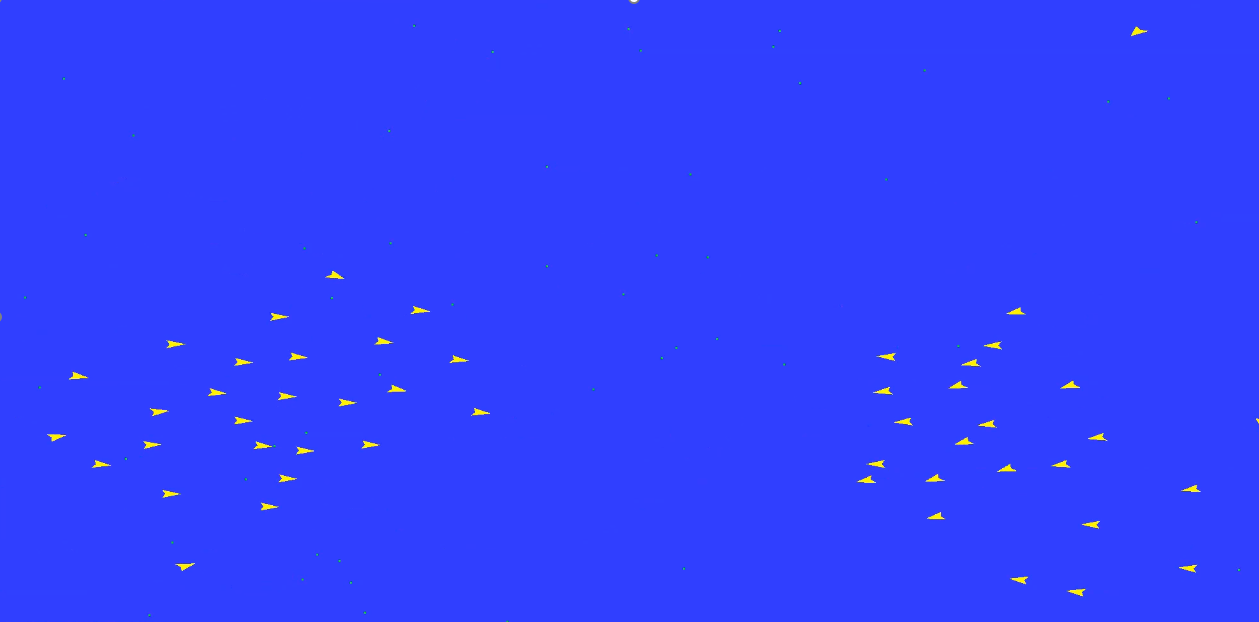
\includegraphics[width=.8\linewidth]{basicFlocks}
  % replacing the above command with the one below will explicitly set
  % the bounding box of the PS figure to the rectangle (xl,yl),(xh,yh).
  % It will also prevent LaTeX from reading the PS file to determine
  % the bounding box (i.e., it will speed up the compilation process)
  % 
\includegraphics[width=.95\linewidth, bb=39 696 126 756]{sampleFig}
  %
  \parbox[t]{.9\columnwidth}{\relax
        This image shows a basic flocking pattern created by the fundamental forces.
           }
  %
  \caption{\label{fig:firstExample}
           Basic Flocking.}
\end{figure}
To fix the Boids turning too rapidly, a solution called "turn rate" was created that would take a portion of the desired velocity update. The system starts with the current velocity of the Boid and the velocity of the boid that was calculated after adding the three fundamental forces. The difference between these vectors is computed to get the change in velocity, which is then scaled by a fraction such as 1/10 to get a portion of the desired velocity change. This change is then added to the current velocity of the Boid to create a final result. This system is ideal because it is simple and computationally inexpensive, but it suffers from creating a variable turn rate depending on the the magnitude of the velocity change. If the Boids desired velocity is significantly different than its current velocity than it will turn faster compared to a Boid that is travelling at a velocity that is close to its desired velocity. If a constant turn rate is desired then the velocity change could be normalized and scaled by a constant using the method described for velocity limiting. For this project, the computation cost of normalizing the turn rate was deemed too expensive so a dynamic turn rate was used.
\subsubsection{Multiple Flocks}
With the basic Boid implementation complete, this system needed to be further extended with the ability to add multiple flocks of Boids. This feature is important for working towards an evolution simultor and provides several other benifits to the overall system. Creating multilpe flocks is a relatively simple procedure that involved splitting the desired number of Boids into several equal sized groups. Each flock then updates its velocity every time step based on nearby members of their own flock. This provides a huge advantage of reducing the number of nearby Boids that each individual Boid needs to consider. The nature of the Boid algorithm is $O(n^2)$ which means that if there are $n$ Boids created then each Boid needs to perform $n$ checks. This means that a system with 1000 boids would need to perform $1000 * 1000 =  1,000,000$ checks per tick. Using an example of 5 flocks we can see how having multiple independant flocks can reduce the number of checks per tick. If the 1000 boids were divided between 5 flocks then each Boid would only need to check 199 other boids. This would result in $200 * 200 * 5 = 200,000$ checks per tick. This simple division creates a 5x improvement in the number of checks that are needed per tick in this case.
\par
It is worth noting that the multiple independant flock approach loses some granular control this is available when all Boids in contained in a single flock. For example, the Boids no longer check separation force between themselves and members of other flocks which means that collisions can occur.
\subsubsection{Predators}
\label{hunting}
In order for evolution to occur, the boids needed a mechanism to determine which Boids were the weakest. This was accomplished by introducting predators into the system that actively hunt and kill Boids. The predator isn't a member of a flock and is therefore not influenced by the flocking forces described in section \ref{forces}. Instead, the predator travels in a straight line until it's hunger increases above 20\% of its maximum hunger amount. Hunger is described in a greater detail in section \ref{hunger}. Once this threshold is reached, the predator switches into a hunting state and will try to catch food. On each step, every predator calculates the closest Boid to its current location and determines the vector between itself and the prey. A portion of that vector is added to the predator's velocity similar to the "turning rate" method described previously. If a predator is within a small range of a Boid, then the boid is killed and the predators hunger bar is reset to 0. 
\par
The Boids were also given a mechanism to escape the predator. Every simulation tick each predator generates a list of Boids that are within its perception radius. A force is then applied to each Boid in the direction of the vector between the predator and the Boid. At first glance this approach seems counter intuitive that the predator is looking for Boids instead of each Boid checking for a list of predators. However, due to the optimization method that will be described in section \ref{qtree}, it was vastly more efficient to check predator interactions in this way and it doesn't change the overall outcome of the simulation.
\subsection{Working as a Flock}
Everything described so far in this project has discussed how flocking behaviour is created, but doesn't provide a motivation for why the Boids should create flocks. This project aimed to provide motivation for the Boids to flock instead of enforcing arbitrary rules on the agents. This section discusses how the Boid behaviour was modified to provide realistic incentives for Boids to group together.
\subsubsection{Herd Safety}
\label{herdImmunity}
In nature, the main reason for birds to flock together is to outnumber predators which increases their survival chance. This project emulated this behaviour by implementing a deterrent for predators hunting habits based on the density of Boids.
\par
An extension of the predator hunter behaviour was created that prevented the predator from perusing Boids that were part of a large local group. The predator looks at Boids one at a time from each flock, starting at the closest and working outwards until a target is found. For each Boid, a radius is drawn around the potential target and a list of Boids that are also members of that flock is returned. The total mass of these boids is added up and compared to a threshold level. If the mass is below the threshold then the predator stops looking for prey and uses that target to calculate a change in velocity as described in section \ref{hunting}. If the total mass is above the threshold then it continues on to the next potential target. The target is recalculated each tick of the simulation which means the predator can search for new prey if its first target is too fast to catch or joins together with a larger group of its flock before the predator can catch it.
\subsubsection{Hunger and Food}
\label{hunger}
The safety in numbers strategy improves the realism of the animation but it violates the goal of not prescribing an optimal strategy. At this point there is no disadvantage to creating large groups and no incentive to leave the group. To fix this problem, a hunger system was introduced that forces Boids to seek food in order to survive. This system works by adding a hunger level to each Boid that is tracked internally along with randomly generated food for the Boids to eat. On every tick of the simulation, the Boid's hunger increases proportionally to its speed. That means that fast Boids will starve faster but are also more likely to be able to outrun a predator. 
\par
Once the Boid's hunger exceeds 20\% of it's maximum hunger, it starts looking for food in its immediate surroundings. This mechanic works similarly to the hunting algorithm of the predators described in section \ref{hunting}. On each simulation step, each Boid that has hunger above the threshold looks for the nearest food to itself. A force is then applied to the Boid in the direction of the food proportional to how hungry the Boid is. The force starts small but grows exponentially as the Boid gets hungrier. This force is added to the fundamental forces from section \ref{forces} before the turning rate and speed limiting are applied.
\subsection{Algorithm Overview}
This section shows pseudocode for the algorithms described in the previous sections. The first algorithm shows a very broad overview of the velocity update on each Boid for each timestep. Note that this algorithm has been simplified and is missing the force calculation for avoiding predators. 
\begin{algorithmic}
\For{Each Boid}
    \State $boid.velocity \gets randomVelocity$
\EndFor
\While{true}
\For{Each Flock}
    \For{Each Boid b in Flock}
        \State $b.hunger \gets b.hunger + 1$
        \State $desiredVel \gets b.velocity$
        \State $desiredVel \gets desiredVel + cohesion$
        \State $desiredVel \gets desiredVel + separation$
        \State $desiredVel \gets desiredVel + alignment$
        \If{b.hunger > 20}
            \State $desiredVel \gets desiredVel + foodForce$
        \EndIf
        \State $velChange \gets desiredVel - b.velocity$
        \State $b.velocity \gets b.velocity + velChange * turnrate$
        \State $b.velocity \gets \frac{b.velocity}{|b.velocity|} * b.turnRate$
    \EndFor
\EndFor
\EndWhile
\end{algorithmic}
\subsection{Evolution}
With all the features in place to facilitate the evolution, the only remaining step was to create a system to spawn new offspring. In nature, populations of predators and prey are kept in balance. When the predator population increases too much then they begin to starve due to lack of food which leads to an explosion in the population of the prey species as the predators die off. This increases in food bolsters the predator population in a cycle until an equilibrium is reached. This system works in nature because habitats are very large which means that finding prey becomes more difficult as the population the of prey species gets lower. However, the simulation in this project is in a small space which means that locating prey is simple. There are no burrows for the prey to hide in or camouflage of any kind. 
\par
Due to the small size of the environment, a straightforward approach was taken. Each time a boid died from starvation or from a predator, a new Boid would be created on the next simulation step. This isn't very realistic, but provides a good enough model for demonstrating evolution without worrying about the entire predator or prey population dying from starvation. This addresses the question of when to create new boids but not how they should be created. Before discussing that topic, the boids needed properties that could evolve. These properties were created as follows:
\begin{enumerate}
    \item Scalar multiplier for cohesion. This multiplies the force that the Boid experiences from cohesion towards other Boids. The cohesion calculation is still computed as discussed in section \ref{forces}, but the total cohesive force is multiplied by the scalar before it is applied to the boid.
    \item Scalar multiplier for separation. This works identically to the scalar for cohesion, but it is applied to the separation force experiences by the Boid.
    \item Scalar multiplier for alignment. This works identically to previous two multipliers but it is applied to the alignment force applied to the Boid.
    \item Speed. This has been references in previous sections but in this section it is turned into a dynamic property of the Boid instead of a constant. The speed of the Boid is added to its hunger every step, resulting in fast Boids starving quicker. However, Boids with higher speed can move faster.
    \item Mass. The mass of a Boid doesn't do anything by itself but it can alter the behaviour of the Boids interacting with a flock. As described in section \ref{herdImmunity}, the predator cannot hunt groups of Boids that are above a certain mass. This mass is calculated by summing the individual masses of each of the Boids in the group. However, the turn rate of the Boids is divided by their mass which results in large Boids turning at a slower rate. This makes it more difficult for them to avoid predators.
\end{enumerate}
The reason for creating these trade-offs was to try to create several viable strategies for the Boids. For example, fast Boids could survive by outrunning the predators with their superior speed and turning rate, while slow Boids with large mass could flock tightly together to prevent the predator from selecting them as a valid target. There is also a tradeoff in separation and cohesion. Tightly separated Boids are more likely to reach the threshold mass required to scare away the predator, but tightly groups Boids are also more likely to be eaten in rapid succession by a predator if the group splits up.
\par
This result seemed much more interesting than a clearly defined result emerging. In the initial prototype, no disadvantage was given for speed which caused the boid speed to increase forever until the simulation looked very unnatural. 
\par
With all the properties of the Boids created, it is finally possible to create evolution. To start, a modification was made to the algorithm described before that initialized each of the flocks with random attributes. Each flock generated a unique set of values in the range from 0.5 to 1.5 for each of the five attributes and then assigned those values to each of its members. If a simulation was initialized with 5 flock, then 5 flocks would be created in which the members in each flock have the same attributes but each have different values than the members of the other flocks.
\par
The simulation is then started and run as described before until a Boid died. At this time two parents need to be selected to create a new Boid. The first parent is chosen by selecting a random Boid from the flock that the Boid died from. The second parent is chosen as a random Boid from any of the other flocks.
\par
Once the parents are selected, a process called crossover occurs \textbf{CITE HERE}. This process involves creating a new Boid with uninitialized attributes and then filling in the values from the parents. In this project, the child has a uniform chance of inheriting each attribute from either parent. This means that on average, the Boid will inherit 50\% of its attributes from one parent and 50\% from the other. However, since there are 5 attributes which each have a 50\% chance of being inherited, there is a $\frac{1}{2^5} = 3.125\%$ chance of the new Boid being an exact duplicate of each parent.
\subsubsection{Mutation}
With crossover complete, the Boids technically evolve, but each time the simulation runs there are only as many possible values for each attribute as there are flocks. This means that simulations with 3 flocks only have $5^3 = 125$ possible Boid permutations. It's possible that none of these permutations is optimal for the provided environment which means a more dynamic system is required. To remedy this, a mutation chance is introduced into the system that gives each attribute a chance to chance slightly when it is inherited from a parent. In this implementation a mutation chance of 10\% was used. After the child randomly selects an attribute from a parent there is a 5\% chance that the inherited value will be increased by 0.1 and a 5\% chance that it will be decreased by 0.1. This system relies heavily on randomness to produce the best result over time through trial and error instead of prescribing an optimal strategy.
\subsection{QuadTrees}
\label{qtree}
All the main mechanics of the system have been discussed at this point, but the performance of the system is lacking. The main problem is the number of entities that each Boid needs to consider to calculate its forces.  At present, each Boid needs to calculate the distance to each other Boid to calculate cohesion, separation and alignment forces. The predator also needs to consider the distance to every Boid form every flock to find the closest target and apply repulsive forces to the Boids.
\par
A solution used for this project involved the introduction of a spacial division data structure called QuadTrees. QuadTrees are a tree based data structure in which each node can contain references to four other nodes, called children nodes. Additionally, the node can contain a list of Boids within it, a center point of the node, and the width/height. Each of these nodes represents a a Axis-Aligned-Bounding-Box (AABB) which occupies a region of the screen. When each tree is initialized, it just has a single root node that contains the entire screen. When the maximum capacity of the root node is exceeded by inserting more than five Boids into it, then the root creates 4 children. Each of these children will occupy 1/4 of the screen in the top-right, top-left, bottom-left, and bottom-right regions and have their own capacity of 5.
\par
When a new Boid is inserted into the tree, the top level node calls the insertion function on each of its children until one of them returns that it was successfully inserted. Each of the children operates identically to the root node in a recursive fashion. When the insert function is called on the child, it checked if the Boid being inserted in contained in it's region. This can be done very easily since the Boid's center is a point mass and the regions of the QuadTrees are AABB. If the Boid is not inside the child then the parent can immediately move on to trying the insert function on the next child. When a child nodes becomes saturated with Boids then it will create children of its own, splitting into four sub-regions.
\par
Once all the Boids are inserted into the QuadTree, the tree can be queried to find all the Boids in a specific region. For this application, the regions are circular areas around each of the Boids that represent their perception radius. The query functions works with the addition of an intersection function that checks if a given region overlaps with a quadTree node. If it does, all the Boids contained by the QuadTree are appended into a list of nearby Boids and the query function is recursively called on the QuadTree's children. Each Boid then checks the distance to each of the Boids in the list returned by the query instead of checking distance to every Boid.
\par
This query function converts the algorithm from a $O( n^2 )$ into a $O(n * log_2{n})$. That means that a system using 1000 Boids would go from computing $1000 * 1000 = 1,000,000$ checks to using $1000 * log_2{1000} \approx 10,000$ which is a 100x performance improvement. The QuadTree was also made to work with generic objects that have a position property. This allowed the food system to use QuadTrees to save on Boids needing to calculate the distance to every item of food.
\section{Evaluation}
In order to evaluate the project, the execution environment must first be understood. For this project, all simulations were compiled and run on a Windows 10 desktop computer with a Ryzen 5 3600 CPU, a RX 5700XT GPU made by AMD, and 16GB of 3600Ghz RAM.
\par
This project contained a large number of input parameters that can be tuned to produce different results. Some of these include the following
\begin{itemize}
    \item The range of default values provided to the Boids for mass, separation, alignment, cohesion and speed.
    \item The perception radius of the predator looking for boids to eat and the perception radius of the Boids looking for food.
    \item The range in which Boids have their fundamental forces altered by other Boids.
    \item The quantity of food in the environment.
    \item The rate at which predators and Boids get hungry.
    \item The threshold value for mass that prevents a predator from targetting a flock of Boids. 
    \item The strength of the force that pushes Boids away from the predator.
    \item The mutation rate used when creating offspring.
    \item The number of Boids and predators at the start.
\end{itemize}
Each of these parameters will effect how the simulation looks and how the properties of the Boids evolve over time. Due to the number of changable parameters and the number of values each of these parameters can have, it is impossible to demonstrate the results for each of them. However, this section will show the results of several hand-picked examples that show general trends to get an idea of how the system works.
\section{Conclusion}
\printbibliography                
\end{document}
